\paragraph{Sơ đồ tuần tự luồng yêu cầu khôi phục mật khẩu}

Luồng nghiệp vụ này mô tả
quy trình người dùng gửi
yêu cầu khôi phục mật khẩu
thông qua địa chỉ email đăng ký
để nhận liên kết xác nhận từ Auth Service.

\begin{figure}[H]
\centering
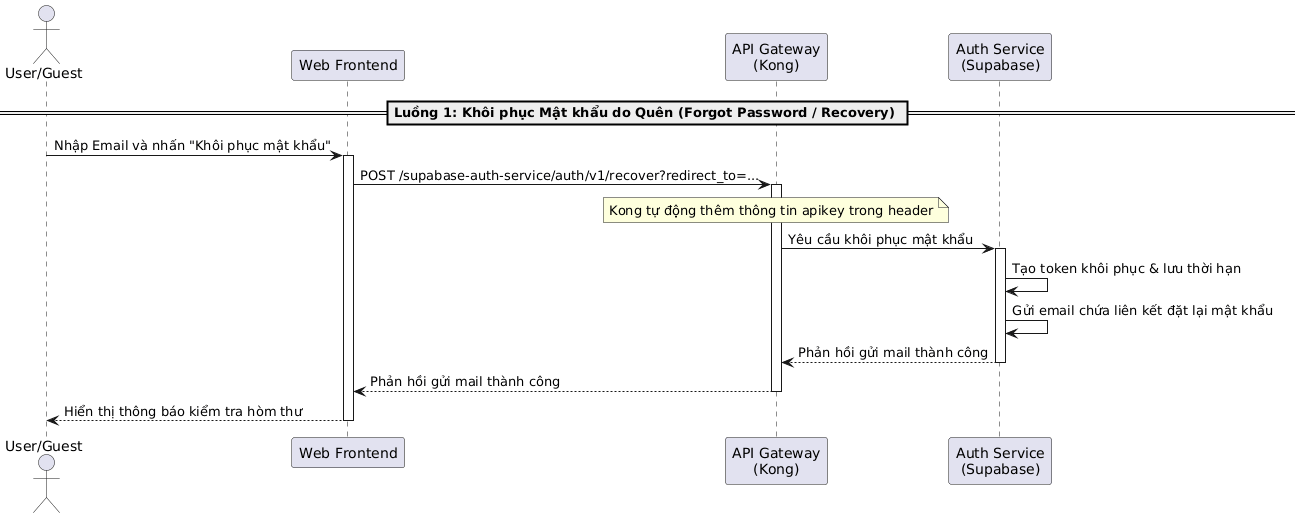
\includegraphics[width=0.95\textwidth]{contents/Sequence/UML-Sequence-UserForgotPasswordRequest.png}
\caption{Sơ đồ tuần tự luồng yêu cầu khôi phục mật khẩu}
\end{figure}

\subparagraph{Mô tả tổng quan}

\begin{itemize}

\item \textbf{Yêu cầu khôi phục:}
Người dùng điền
địa chỉ thư điện tử và nhấn nút yêu cầu khôi phục mật khẩu.
Giao diện gửi yêu cầu khôi phục qua cổng API đến Auth Service.

\item \textbf{Gửi email liên kết:}
Auth Service tự tạo mã khôi phục mật khẩu,
ghi nhận thời hạn sử dụng của mã này và
trực tiếp gửi một thư điện tử chứa đường dẫn liên kết
đặt lại mật khẩu đến thư điện tử của người dùng.
\end{itemize}

\begin{table}[H]
\centering
\renewcommand{\arraystretch}{1.3}

\begin{tabular}{|l|l|p{5cm}|}
\hline
\textbf{Thành phần} & \textbf{Phân loại} & \textbf{Vai trò trong hệ thống} \\ \hline
User/Guest & Actor & Người dùng hoặc khách yêu cầu khôi phục mật khẩu. \\ \hline
Web Frontend & Component & Giao diện web Next.js. \\ \hline
API Gateway (Kong) & Component & Cổng API chuyển tiếp các yêu cầu API. \\ \hline
Auth Service (Supabase) & Microservice & Dịch vụ thực hiện xác thực, quản lý token khôi phục và gửi email khôi phục mật khẩu. \\ \hline
\end{tabular}
\caption{Các thành phần tham gia luồng yêu cầu khôi phục mật khẩu}
\end{table}
